Se puede clonar el repositorio desde la página del mismo en \href{https://github.com/codeurjc-students/2024-Atra}{\uline{GitHub}\footnote{\url{https://github.com/codeurjc-students/2024-Atra}}}. Navegando a la pestaña "$<$ $>$ Code", haciendo clic en el botón desplegable "$<$ $>$ Code" encima del listado de archivos, a la derecha, y seleccionando una de las varias opciones ofrecidas.

\begin{figure}[H]
    \centering
    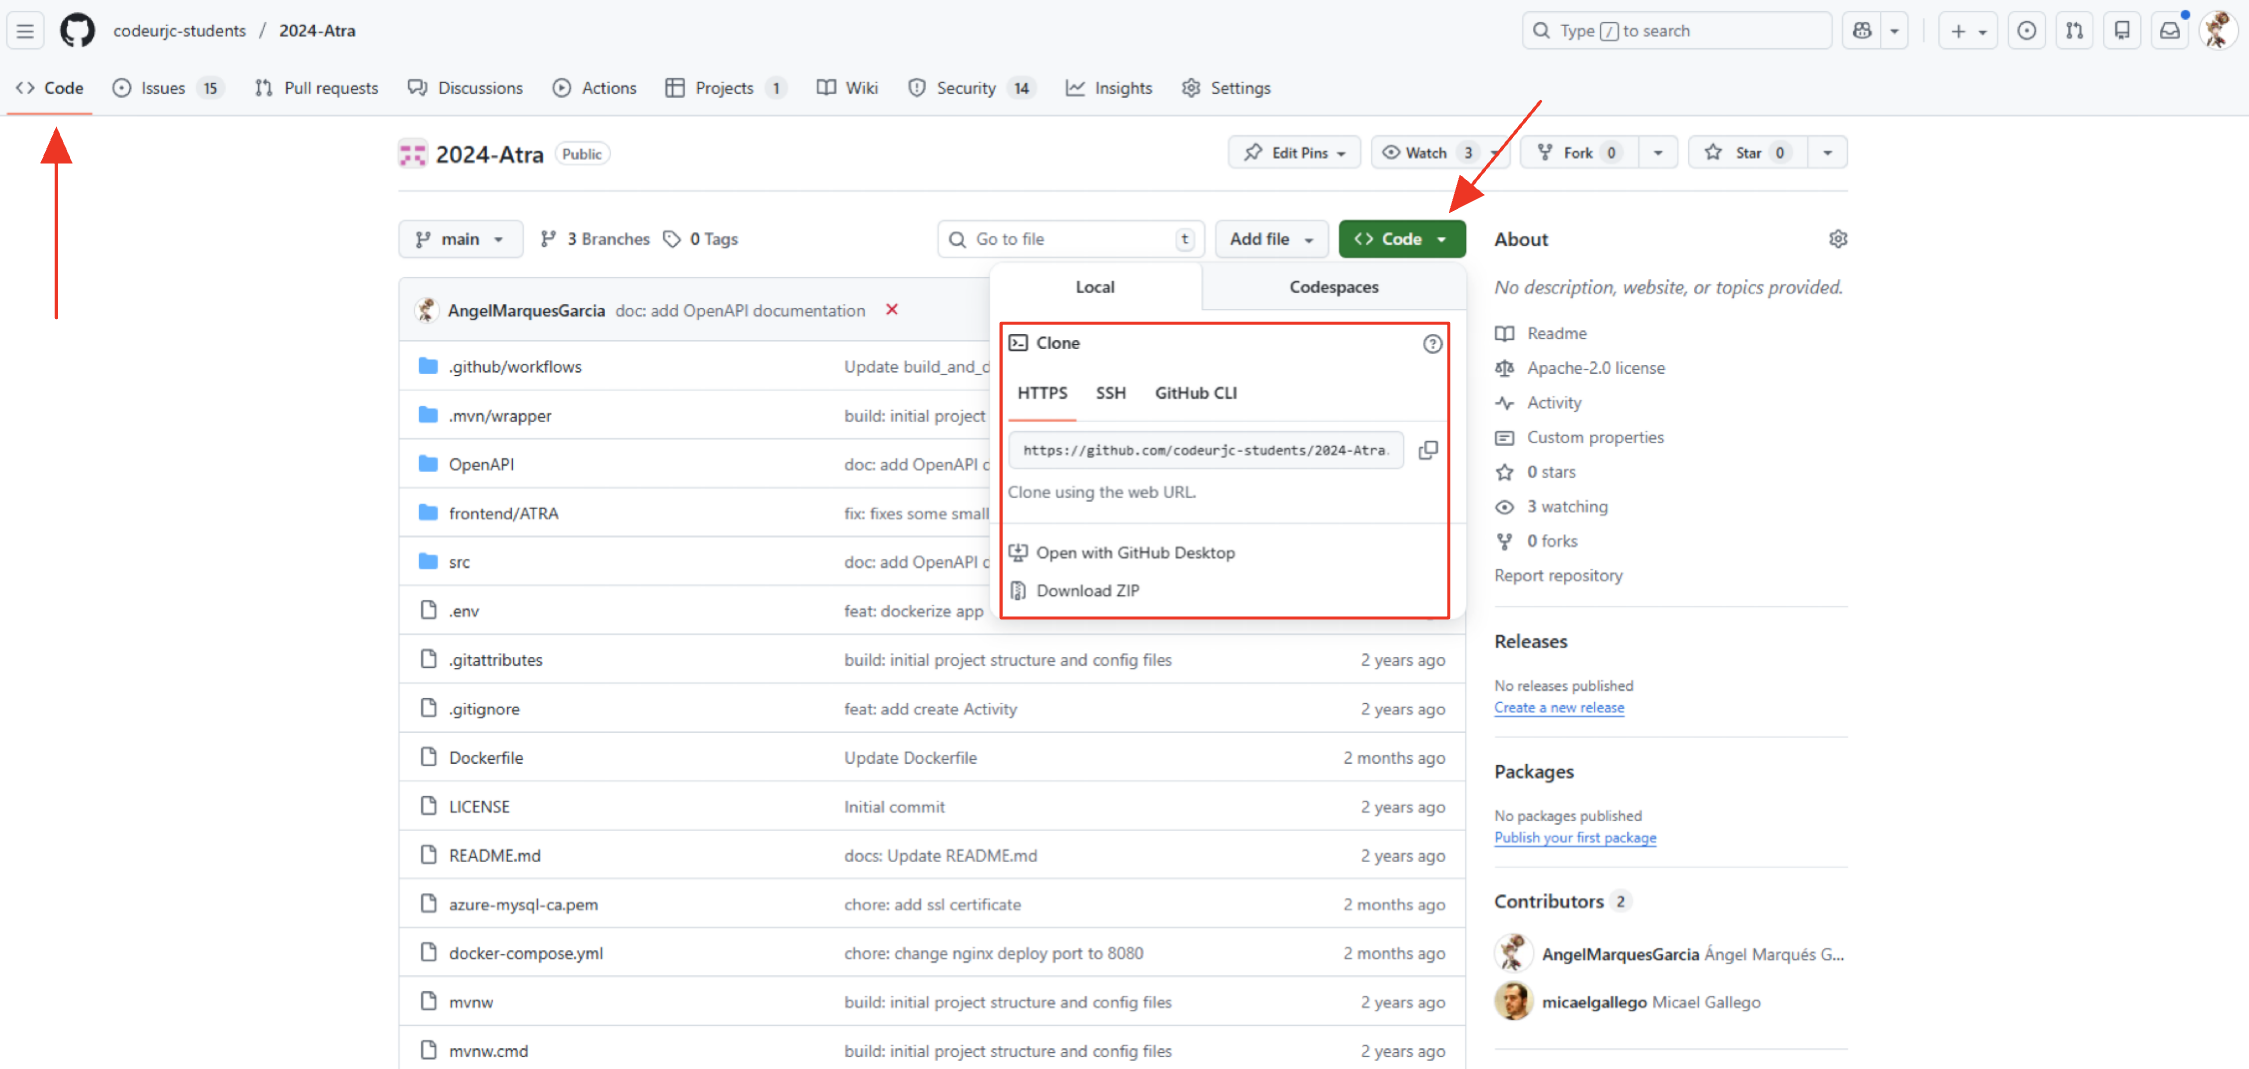
\includegraphics[width=1\linewidth]{img/instrucciones_clonar_repo.png}
    \caption{Instrucciones para clonar el repositorio}
    \label{fig:clonar_repo}
\end{figure}

\section{Ejecución de la aplicación}
Una vez clonado el repositorio, se puede proceder a ejecutar las distintas partes del código. 
\subsection{Base de datos}
Es necesario crear el schema de la base de datos antes de poder ejecutar la aplicación. Una vez creada no es necesario volverla a crear a no ser que se elimine manualmente. Aunque la aplicación se pare y se ejecute varias veces, no será necesario volver a crear el schema. Sólo será necesario que el servicio de MySQL esté en ejecución

Para crear la base de datos es necesario tener MySQL descargado. Se puede descargar desde \href{https://dev.mysql.com/downloads/installer/}{\uline{esta página}\footnote{\url{https://dev.mysql.com/downloads/installer/}}}. Una vez instalado, debemos asegurarnos de que el servidor esté en ejecución. La forma de hacer esto depende del sistema operativo:
\begin{itemize}
    \item Windows: pulsar tecla de windows + r, escribir services.msc, y pulsar aceptar. Esto abre la aplicación Servicios. Buscamos el servicio MySQL, y comprobamos que esté en ejecución. Si no lo está, se puede arrancar con clic derecho, iniciar.
    \item Mac: se puede comprobar el estado ejecutando el comando \texttt{mysql.server status} en la terminal. Si no está en ejecución, lo arrancamos con \texttt{mysql.server start}.
    \item Linux: se puede comprobar el estado ejecutando el comando \texttt{sudo systemctl status mysql} en la terminal. Si no está en ejecución, se puede arrancar con \texttt{sudo systemctl start mysql}.
\end{itemize}

Una vez el servidor de MySQL está en ejecución deberemos crear el Schema para la aplicación. Para ello, debemos ejecutar en terminal el comando \texttt{mysql -u root -p}, seguido de \texttt{CREATE DATABASE atra;} en el prompt de sql, para crear el Schema. Una vez creado el Schema ya se puede ejecutar la aplicación.

\subsection{Backend}
El \textit{backend} se puede ejecutar de varias maneras distintas. Podemos ejecutarlo desde la consola navegando a la carpeta 2024-ATRA (que contiene la carpeta src), y ejecutar el comando \texttt{mvn spring-boot:run}. Esto compilará y ejecutará la aplicación, pero no crea un archivo .jar persistente. Es equivalente a lanzar la aplicación desde un IDE. Alternativamente, podemos ejecutar el comando \texttt{mvn clean package -DskipTests} para compilar y empaquetar la aplicación. Esto genera un archivo .jar que podemos ejecutar con \texttt{java -jar target/ATRA-1.0.0-SNAPSHOT.jar}. El nombre del jar depende del artifactID y version incluidos en el pom.xml. Siempre será \texttt{<artifactID>-<version>}

Alternativamente, como se ha mencionado, se puede abrir el proyecto con un IDE y ejecutarlo a través del mismo.

\subsection{Frontend}
El \textit{frontend} se puede ejecutar navegando a la carpeta /frontend/ATRA en la terminal, y lanzando el comando "ng serve". Esto lanza el \textit{frontend} en modo desarrollo, de forma que la página se actualizará cuando haya cambios a los archivos. 

\section{Herramientas utilizadas durante el desarrollo}

\subsection{IntelliJ}
Se puede descargar en la \href{https://www.jetbrains.com/es-es/idea/download/}{\uline{página oficial}\footnote{\url{https://www.jetbrains.com/es-es/idea/download/}}}. Ha sido la herramienta utilizada para desarrollar el \textit{backend}.

Para editar o ejecutar el proyecto con IntelliJ necesitaremos abrir el proyecto. Para ello, clonamos el repositorio desde github o nos descargamos el proyecto como un zip, y abrimos IntelliJ.

Al abrir IntelliJ, asumiendo que no tuviéramos un proyecto abierto previamente, nos mostrará una pantalla como la de la figura \ref{fig:inicio_intelliJ}. Aquí veremos una lista de proyectos recientes, junto con botones para crear uno nuevo o abrir un proyecto existente. En mi caso, el proyecto se encuentra en los proyectos recientes, pero sigue siendo posible abrirlo mediante el botón \textit{Open} en la parte superior de la pantalla. 
\begin{figure}[H]
    \centering
    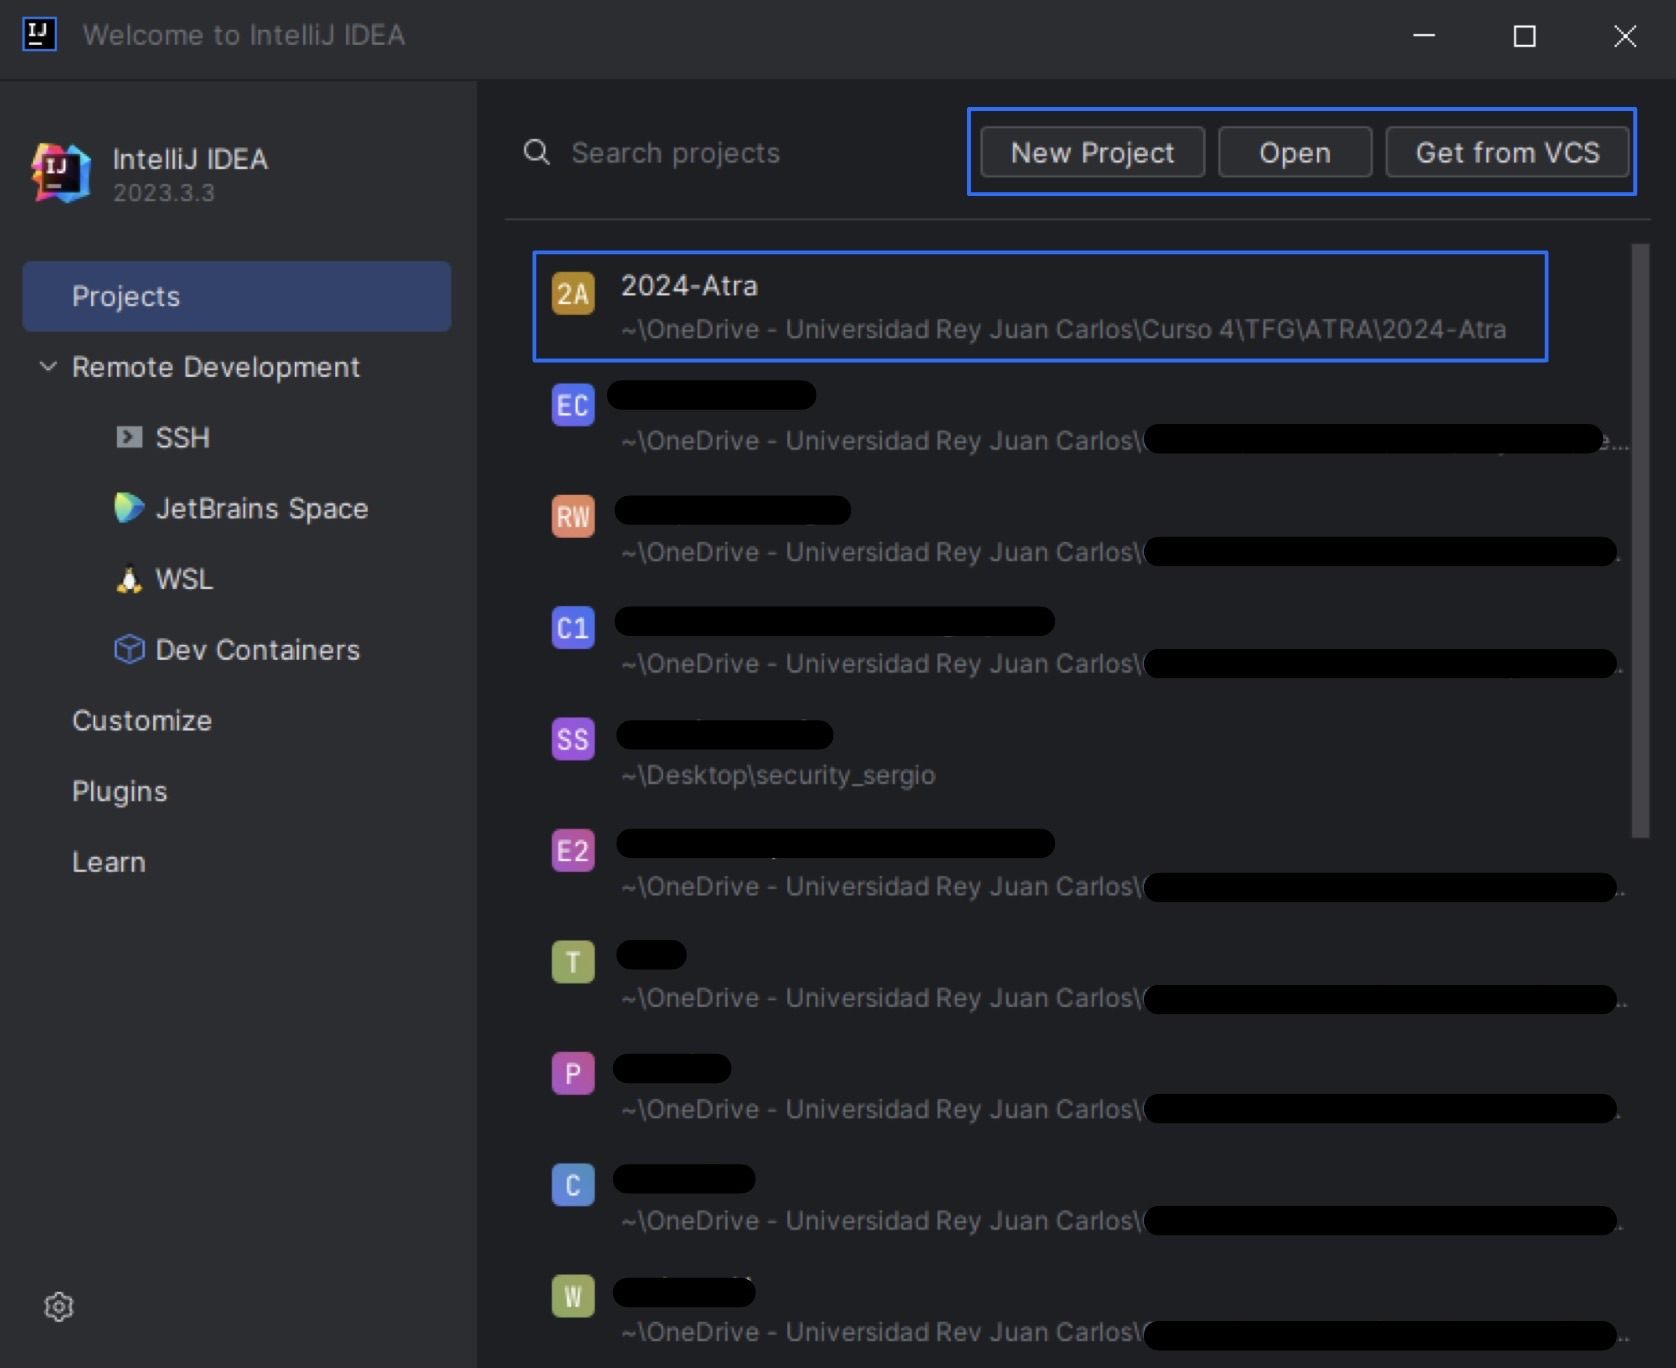
\includegraphics[width=0.5\linewidth]{img/abrir_proyecto.png}
    \caption{Pantalla de inicio IntelliJ}
    \label{fig:inicio_intelliJ}
\end{figure}

Al pulsar en Open nos permitirá seleccionar una carpeta. Cuando identifique una carpeta que contiene un proyecto de intelliJ la marcará con un icono especial. Deberemos seleccionar la carpeta 2024-Atra, raíz del repositorio.
\begin{figure}[H]
    \centering
    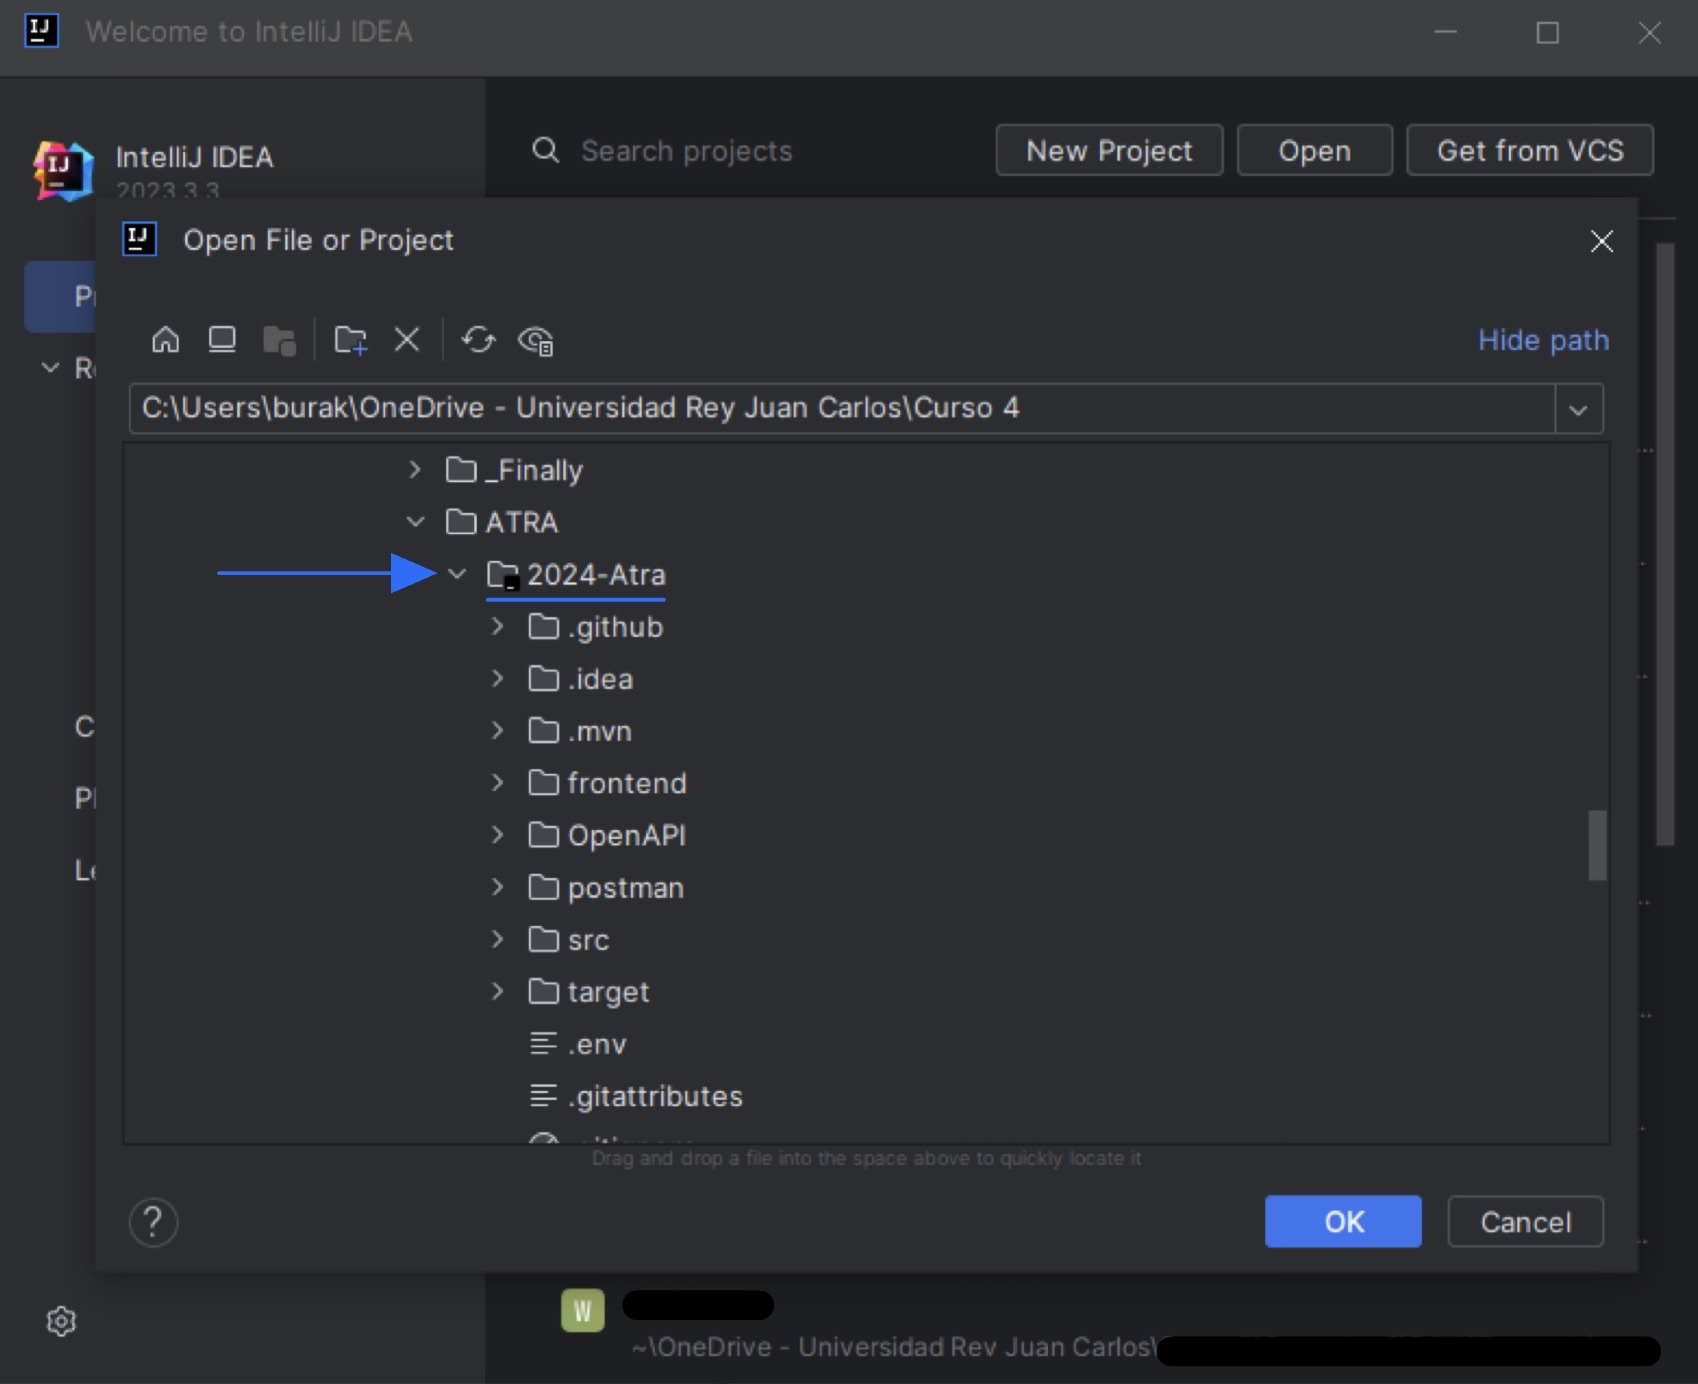
\includegraphics[width=0.5\linewidth]{img/select_project_ij.png}
    \caption{Seleccionar Proyecto en IntelliJ}
    \label{fig:select_project_ij}
\end{figure}
Una vez abierto el proyecto, tendremos una vista como la indicada en la figura \ref{fig:project_view_ij}. Podremos navegar por los archivos del proyecto mediante el menú lateral, marcado como 1. Cuando seleccionemos un archivo, se mostrará su contenido en la ventana principal, a la derecha del menú lateral. Podremos ejecutar el archivo actual o distintas configuraciones mediante los botones en la sección marcada 2 (parte superior derecha). Podemos ver la configuración seleccionada en el desplegable a la izquierda, en este caso es "emptyDemo". Si hacemos clic sobre el nombre podremos seleccionar otras configuraciones, así como modificarlas o crear nuevas. Pulsando el botón de \textit{play} ejecutaremos la configuración seleccionada, mientras que si pulsamos el botón a la derecha, con forma de bicho, lo ejecutaremos en modo debug. El menú permite ejecutar el código de formas adicionales, así como configurar o eliminar la configuración seleccionada. Por último, la sección inferior marcada como 3 muestra distintas herramientas, que se pueden seleccionar mediante los iconos inmediatamente a su izquierda. En este caso está mostrando una terminal integrada, desde la que podremos ejecutar comandos sin tener que abrir una terminal aparte.
\begin{figure}[H]
    \centering
    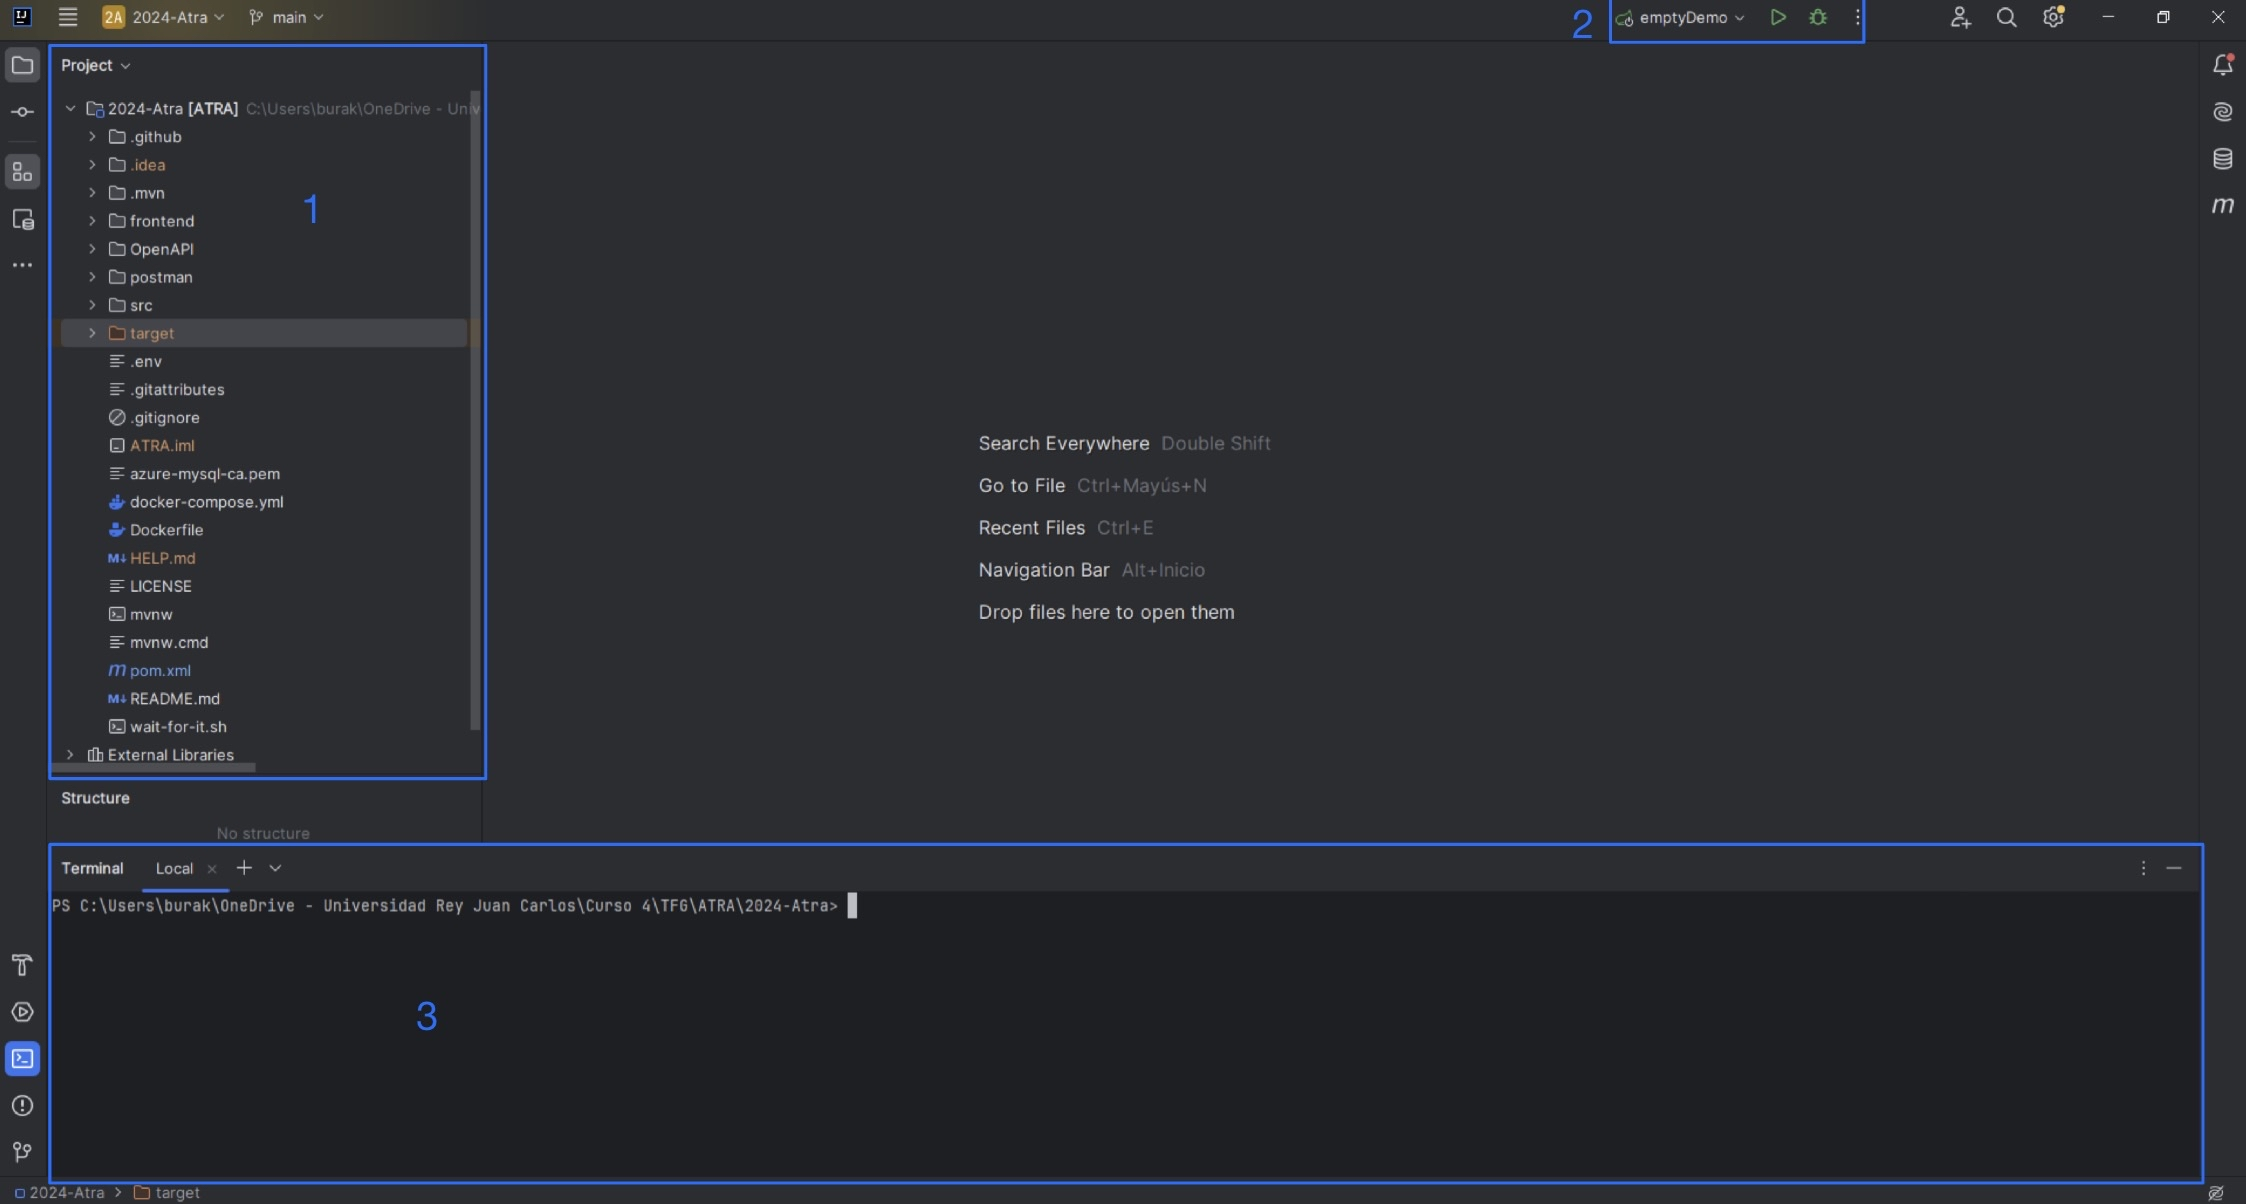
\includegraphics[width=1\linewidth]{img/ij_proyecto_abierto.png}
    \caption{Visión de proyecto en IntelliJ}
    \label{fig:project_view_ij}
\end{figure}

\subsection{Visual Studio Code}
Se puede descargar en la \href{https://code.visualstudio.com//}{\uline{página oficial}\footnote{\url{https://code.visualstudio.com//}}}. Ha sido la herramienta utilizada para desarrollar el \textit{frontend}. 

Igual que con IntelliJ, necesitaremos tener el proyecto descargado. Cuando abramos Visual Studio Code (VSCode en adelante), nos mostrará una pantalla como la de la figura \ref{fig:start_vscode}
\begin{figure}[H]
    \centering
    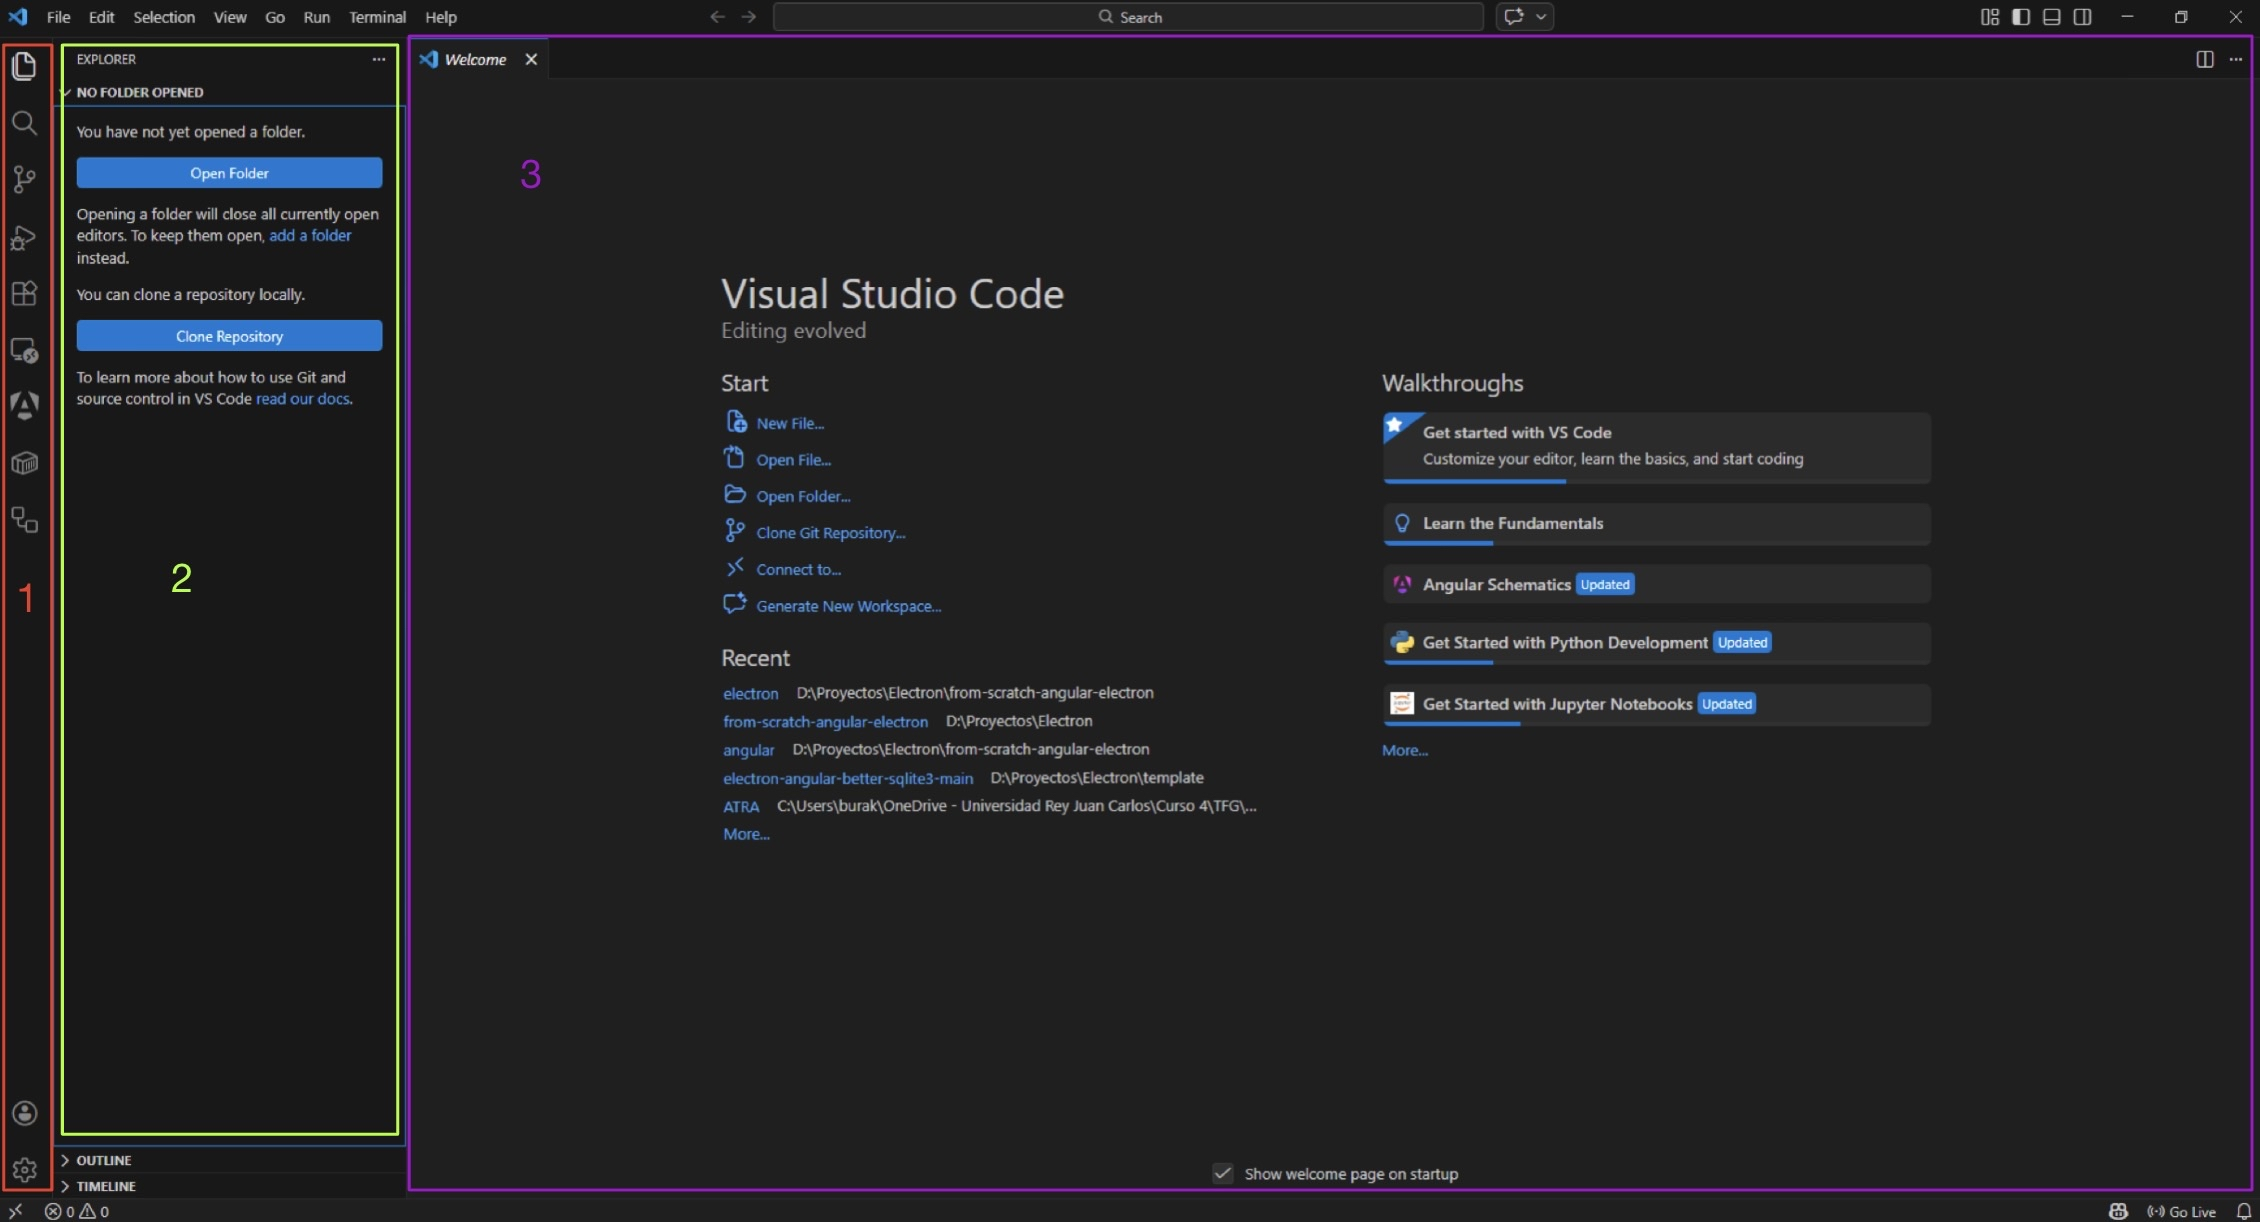
\includegraphics[width=1\linewidth]{img/welcome_vscode.png}
    \caption{Pantalla de Inicio VSCode}
    \label{fig:start_vscode}
\end{figure}

Desde aquí podemos ver la estructura básica del editor. La parte izquierda, delimitada en rojo y marcada como 1 muestra una serie de herramientas configurables. La herramienta seleccionada se mostrará en la sección en verde marcada con 2, o, si no hay ninguna herramienta seleccionada, la sección 2 colapsa para dejar más espacio al editor. Cuando se abra un archivo, o contenido de otro tipo, se mostrará en la sección 3, marcada en morado. Como no hay ningún proyecto, nos invita a abrir uno. Podemos hacerlo de varias maneras, seleccionando "Open Folder" en la ventana abierta en la zona 3, en el botón de la sección 2, o mediante el menú superior yendo a \texttt{file -> open folder}. Es posible que la sección 2 no sea visible de primeras. Si este fuera el caso se puede abrir seleccionando el primer icono de la zona 1. 

Para abrir el proyecto deberemos navegar a la raíz del repositorio y seleccionar la carpeta que contiene el proyecto de frontend, que es /2024-Atra/frontend/ATRA. Cuando abramos el proyecto, la sección 2 se poblará con los archivos y carpetas del proyecto seleccionado, como se puede ver en la figura \ref{fig:proyecto_abierto_vscode}
\begin{figure}[H]
    \centering
    \begin{minipage}{0.48\linewidth}
        \centering
        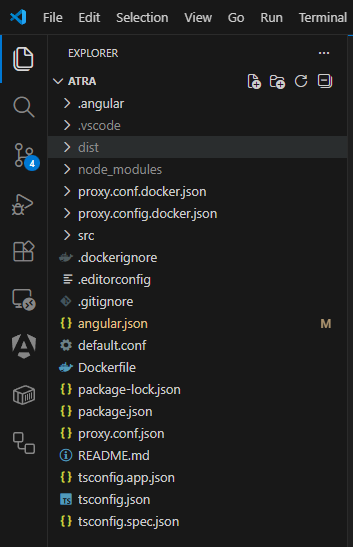
\includegraphics[width=\linewidth]{img/proyecto_abierto_vscode.png}
        \caption{Vista de proyecto en VSCode}
        \label{fig:proyecto_abierto_vscode}
    \end{minipage}
    \hfill
    \begin{minipage}{0.48\linewidth}
        \centering
        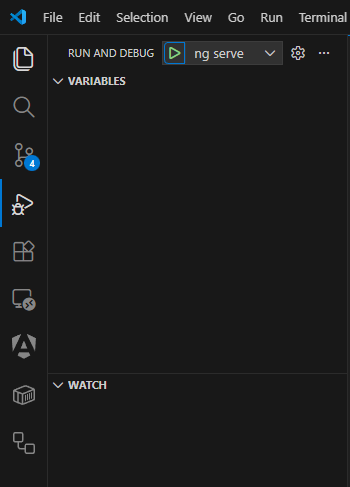
\includegraphics[width=\linewidth]{img/debug_vscode.png}
        \caption{Debugger en VSCode}
        \label{fig:debug_vscode}
    \end{minipage}
\end{figure}
Podremos ejecutar el código pulsando f5 o navegando en el menú lateral a la sección run \& debug (mostrada en la figura \ref{fig:debug_vscode}). Desde esta sección, podemos seleccionar la configuración a ejecutar, y tendremos acceso a varias herramientas de debugging. 

El atractivo principal de VSCode es su amplia oferta de extensiones. Para instalarlas, debemos navegar a la sección de extensiones en el menú lateral (icono inmediatamente inferior al de ejecución, marcado con 4 cuadrados, uno de los cuales está ladeado), desde donde podremos ver y gestionar extensiones instaladas, así como buscar e instalar extensiones nuevas.

\subsection{MySQL Workbench}
MySQL Workbench es una interfaz gráfica que permite conectarse a servidores MySQL para ejecutar consultas  y operaciones sobre bases de datos y schemas. Para poder usarlo, es necesario crear una conexión al servidor de MySQL en cuestión, para lo cual es necesario hacer clic en el botón de + a la izquierda de "MySQL Connections", en la página principal. Esto abre una ventana desde la cual podemos configurar la nueva conexión, poniéndole un nombre, definiendo el método de conexión, y pudiendo configurar una variedad de parámetros, como el host de la base de datos, el puerto a través del que conectarse, el nombre de usuario y contraseña necesarios para acceder, y otras configuraciones más avanzadas. La figura \ref{fig:mysql_workbench} ilustra este proceso.

\begin{figure}[H]
    \centering
    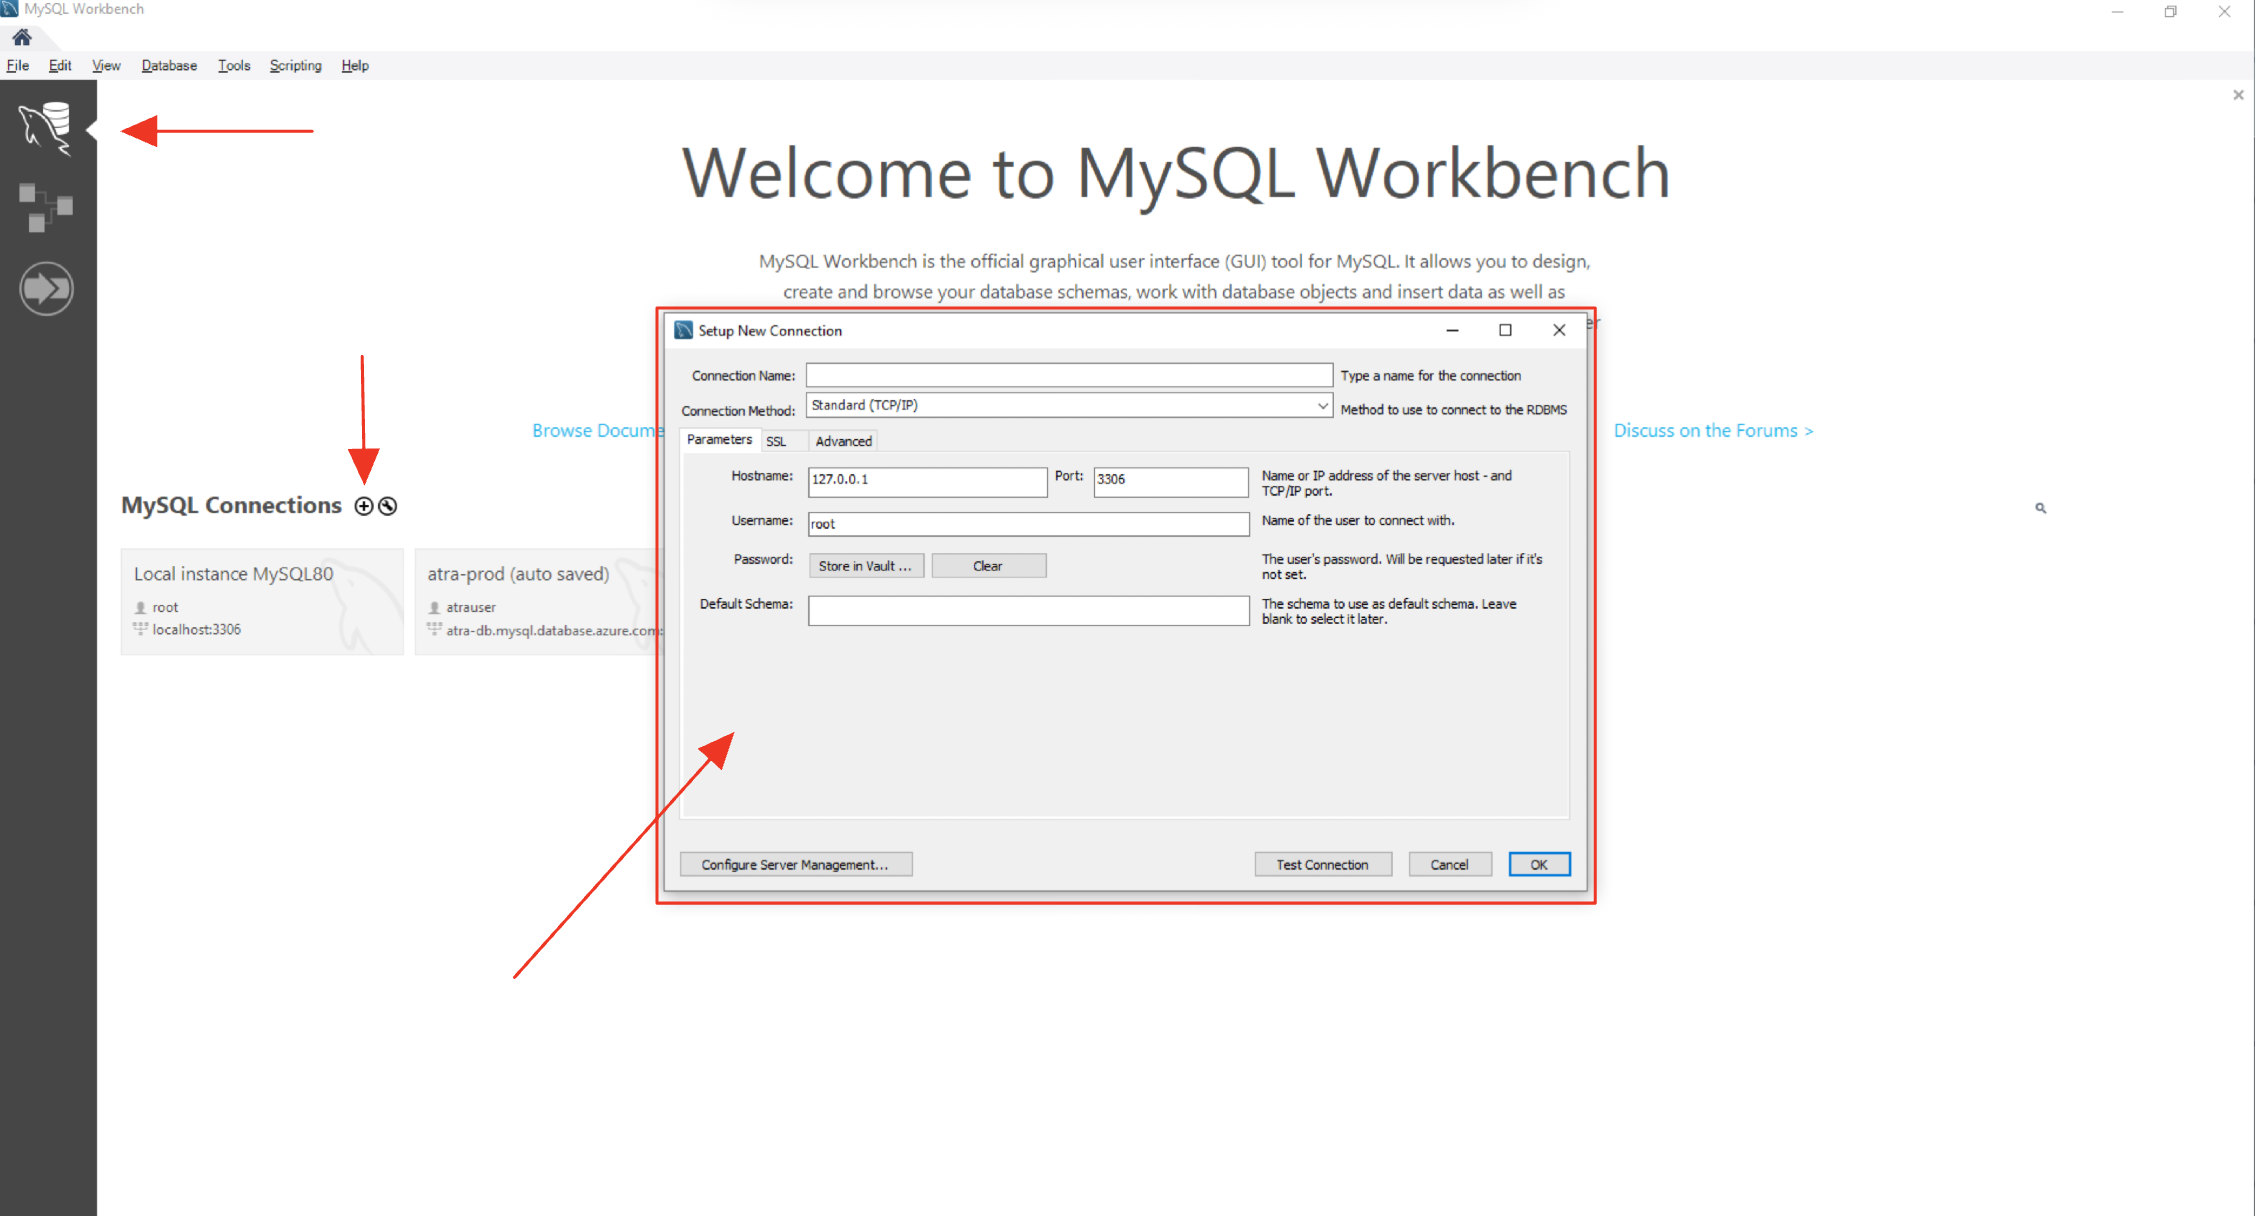
\includegraphics[width=1\linewidth]{img/mysql_workbench.png}
    \caption{Crear Conexión en MySQL Workbench}
    \label{fig:mysql_workbench}
\end{figure}

Para conectar con el servidor de MySQL ejecutado en local, deberemos cambiar el nombre de usuario y contraseña para que coincidan con lo establecido durante la configuración del servidor, y podremos dejar el hostname y puerto como están. Podemos comprobar que los parámetros son correctos haciendo clic en el botón \textit{Test Connection} en la parte inferior del modal. Esto intentará conectarse a la instancia del servidor, y nos informará de si la conexión es exitosa. Es importante asegurarse antes de probar la conexión de que el servidor esté en ejecución, o fallará automáticamente. Si la conexión es exitosa, podemos darle un nombre y crearla pulsando en OK.

Si fuera necesario conectarse a una instancia de MySQL en ejecución en una máquina ajena también será posible, aunque deberemos saber la url en la que está disponible, y el resto de información sobre la conexión, como los usuarios y contraseña permitidos, si es necesario un certificado SSL, etc. Introduciendo esta configuración correctamente, podremos conectarnos a instancias de MySQL remotas. Por ejemplo, durante el despliegue se ha configurado una conexión con la base de datos desplegada en Azure, usando el hostname de la misma: atra-db.mysql.database.azure.com. Es posible que este hostname no esté disponible para conexiones por problemas con el saldo de Azure. 

Una vez se ha establecido una conexión con un servidor MySQL, podremos hacer clic en la conexión creada, y veremos una pantalla como la siguiente:
\begin{figure}[H]
    \centering
    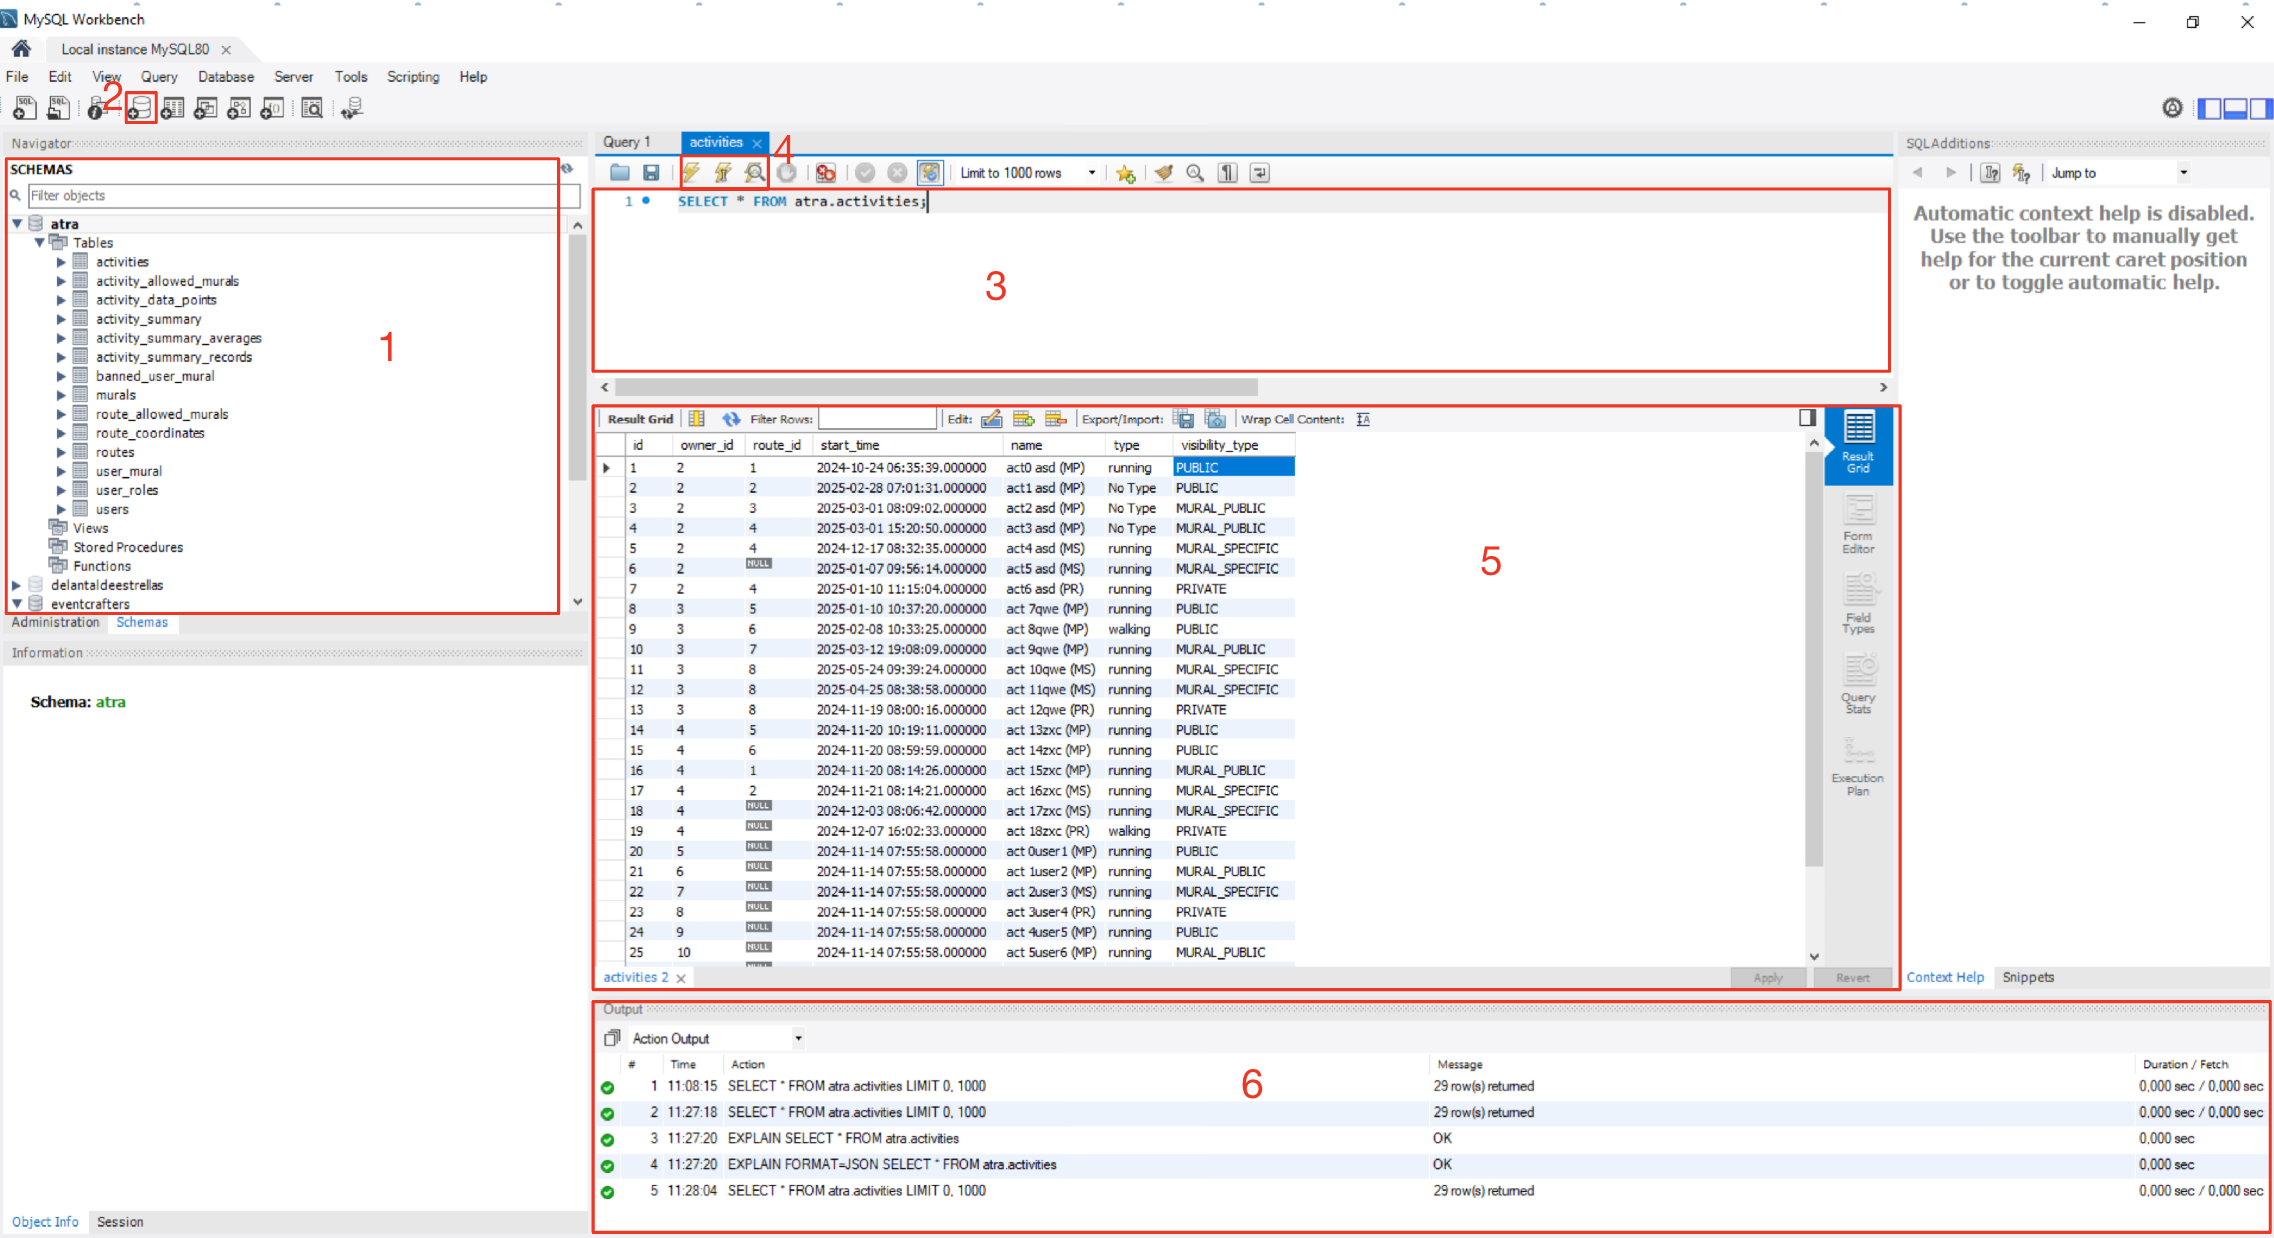
\includegraphics[width=1\linewidth]{img/mysql_conexion_creada.png}
    \caption{Vista de conexión en MySQL Workbench}
    \label{fig:MySQL_conexion}
\end{figure}
La figura \ref{fig:MySQL_conexion} muestra una captura de pantalla de MySQL workbench una vez hemos creado y accedido a una conexión, resaltando y numerando una serie de áreas y botones, para facilitar su explicación.

Lo primero que nos debe llamar la atención es la sección 1. Aquí se muestran los distintos schemas (bases de datos) que existen en el servidor conectado. Podemos ver que en este caso tenemos acceso a las bases de datos "atra", "delantaldeestrellas", y "eventcrafters". Corresponden al proyecto actual y otros proyectos llevados a cabo durante la carrera. Adicionalmente, cada uno de estos schemas es un desplegable. Si lo abrimos, nos mostrará varias secciones. La de mayor interés es la sección Tables, que se encuentra abierta para el proyecto atra. Aquí podemos ver todas las tablas del schema. Podemos hacer operaciones sobre ellas haciendo clic derecho. Adicionalmente, podemos ver que las tablas también son desplegables. Si las abrimos, podremos ver sus columnas, índices, etc.

Sin embargo, es muy posible que cuando accedamos a la conexión no encontremos nada en esta sección, ya que no se haya creado nada todavía. Si este es el caso, podremos crear una nueva base de datos o schema haciendo clic sobre el botón marcado con 2. Esto abrirá una nueva pestaña desde la cual podremos configurar la nueva base de datos a crear. Alternativamente podemos crearla mediante instrucciones SQL.

Para ejecutar instrucciones deberemos introducirlas en la sección marcada como 3. Podremos escribir tantas como queramos, y para ejecutarlas deberemos usar uno de los botones marcados en la sección 4. El botón izquierdo ejecuta todas las instrucciones del editor, o, si previamente hemos seleccionado un subconjunto, ejecutará las instrucciones en ese subconjunto. El botón central ejecutará únicamente la instrucción sobre la que esté posicionado el cursor. El botón de la derecha ejecuta el comando \texttt{EXPLAIN} sobre la instrucción en la que se encuentre el cursor, ofreciendo información sobre el mismo.

Cuando ejecutemos una operación, los resultados de la misma se mostrarán en la sección marcada 5. En este caso, vemos un listado de filas de la tabla "Activities". Adicionalmente, podremos ver un resumen de las instrucciones ejecutadas junto con información sobre las mismas en la sección marcada 6.

\subsection{Postman}
Postman es una herramienta que permite realizar peticiones a endpoints de APIs REST. Permite probar el correcto funcionamiento de los distintos endpoints. Debido al desarrollo paralelo de front y back, no ha sido necesario utilizar postman a menudo, ya que se ha podido confirmar el funcionamiento de los endpoints desde el \textit{frontend}. Sin embargo, sí ha sido utilizado en contadas ocasiones, para solucionar errores persistentes, para determinar si el error viene dado por el front o el back.

En el funcionamiento básico de postman, se crean peticiones que se agrupan en colecciones (\textit{collections}). Al crear una petición se puede determinar el método que utiliza, y se debe introducir la URL a la que irá dirigida. Si la petición debe incluir un cuerpo, podremos cumplimentarlo en la sección "Body". Luego, permite añadir información adicional a las peticiones, como cookies, parámetros, tokens u otros métodos de autenticación, así como los headers de la petición. Cuando se ejecute la petición, muestra los resultados, permitiendo visualizar el cuerpo de la respuesta, así como sus headers y las cookies que tenga asociadas.
